\subsection{Differenzialquotient MOMENTANE Änderungsrate }

\hfill \break
Die errste Ableitung einer Linearen Funtion ist immer die Steigung jener Funtion.\\
Beispiele sind zum Beispiel: Temperaturänderungen, Straßenverlauf, Geschwindigkeit, ...

\hfill \break
Die Sekante ist eine Gerade, die an zwei Punkten den 
Graphen schneidet.\\

\hfill \break
Grundformel: $\frac{\Delta y}{\Delta x} = \frac{f(b) - f(a)}{b - a}$

\hfill \break
Example:\\
Die Höhe eines lotrecht nach oben geworfenem Stein (in m) zum Zeitpunkt t (in Sekunden) ist gegeben
durch die Gleichung $s(t) = 34t- 5t^2$\\
\begin{itemize}
    \item Berechne die mittlere Geschwindigkeit \begin{enumerate}
              \item im Intervall [0; 2]
              \item im Intervall [4; 6]
          \end{enumerate}
    \item  Um wie viel Meter ändert sich jeweils die Höhe?
    \item Wie lange dauert es, bis der Stein wieder auf dem Boden auftrifft?
\end{itemize}

\fboxrule=0.8pt \fcolorbox{lightgray}{lightgray}{
    \begin{tabular}{c}
        (1.)                                                               \\
        \hline
        \\
        Interval [0; 2]                                                    \\
        $\frac{S(2)-S(0)}{2-0} = \frac{48-0}{0} = 24m/s$                   \\
        \\
        Interval [4; 6]                                                    \\
        $\frac{S(6)-S(4)}{6-4} = \frac{24-56}{2} = \frac{-32}{2} = -16m/s$ \\
        \\
        \\
        (2.)                                                               \\
        \hline
        \\
        $S(6) = 34 * 6 - 4 * 6^2$                                          \\
        $S(6) = 204-180 = 24$                                              \\
        $S(6) = 34-4 - 5 *4^2$                                             \\
        $S(6) = 136 -80 = 56$                                              \\
        \\
        \\
        (3.)                                                               \\
        \hline
        Dies kann mit dem Taschenrechner durch ermittlung der Nullstellen errechnet werden.
    \end{tabular}}

\newpage
\hfill \break
Geometrische Interpretation der mittleren Änderungsrate:\\
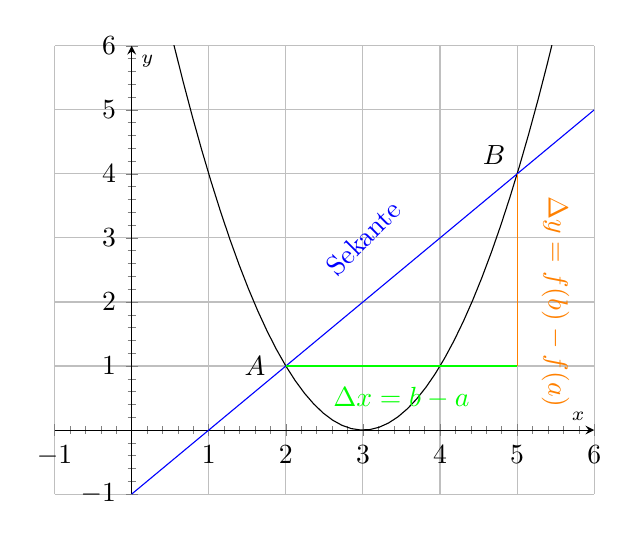
\begin{tikzpicture}[scale=1]
    \begin{axis}%
        [
            grid=major,
            xtick={-1,0,...,7},
            minor x tick num=4, % 4 minor ticks => 5 subintervals
            xmin=-1,
            xmax=6,
            xlabel={\scriptsize $x$},
            axis x line=middle,
            ytick={-1,0,...,7},
            minor y tick num=4,  % 4 minor ticks => 5 subintervals
            ymin=-1,
            ymax=6,
            ylabel={\scriptsize $y$},
            axis y line=middle,
            no markers,
            samples=100,
            domain=-6:6,
        ]
        \addplot[black] (x,{(x-3)^2});
        \draw[blue] (6,5) -- (0,-1);
        \node[color=blue,rotate=45] at (3,3) {Sekante};
        \draw[orange] (5,4) -- (5,1);
        \node[color=orange,rotate=-90] at (5.5,2) {$\Delta y = f(b) - f(a)$};
        \draw[green] (2,1) -- (5,1);
        \node[color=green] at (3.5,0.5) {$\Delta x = b - a$};
        \node[color=black] at (1.6,1) {$A$};
        \node[color=black] at (4.7,4.3) {$B$};
    \end{axis}
\end{tikzpicture}